\documentclass[../main.tex]{subfiles}

\begin{document}

\chapter{Light Ion Interaction Physics}
The mathematical models introduced and derived in the previous two chapters form the basis for our model of the transport of energetic light ions in ICF plasma. In this and the following chapters the interaction physics and multigroup data describing the interactions of light ions as they slow down are discussed. This data will then be combined with our mathematical models to solve light ion transport equations in ICF applications.

A general collision between an incident energetic light ion of species $x$ and a target charged particle of species $T$ resulting in species $s$ and $r$ is written as
\begin{equation} \label{eqn:general-collision}
    x+t \rightarrow r+s \equiv T(x,s)R,
\end{equation}
where particles $s$ and $R$ are termed the scattered and recoiling particles. The general differential cross section that describes the collision in Eq. \eqref{eqn:general-collision} is
\begin{equation} \label{eqn:differentialCrossSection}
    \sigma_{x,t \rightarrow s}(E^{\prime} \rightarrow E; \mucm),
\end{equation}
where the incident ion, $x$, had energy $E^{\prime}$ in the laboratory (LAB) frame of reference before its collision with the target species $t$. The resulting species $s$ is scattered through an angle whose center of mass (CM) cosine is $\mucm$ and has resulting energy $E$ in the LAB frame of reference. The differential cross section in Eq. \eqref{eqn:differential cross section} is a microscopic differential cross section and has units of $cm^{2}$, and is related to the macroscopic differential cross section as
\begin{equation}
    \Sigma_{x,t \rightarrow s}(E^{\prime} \rightarrow E; \mucm) = \mathcal{N} \sigma_{x,t \rightarrow s}(E^{\prime} \rightarrow E; \mucm),
\end{equation}
where $\mathcal{N}$ is the number density of the target species in $cm^{-3}$.

From Eqs. \eqref{eqn:general-collision} and \eqref{eqn:differentialCrossSection}, collisions where the resulting species is identical to the incident species, $s = x$, are termed elastic scattering collisions; and collisions where the resulting species differs from the incident species, $s \neq x$, are termed nuclear-reaction collisions. These nuclear-reaction collisions result in the destruction of the incident ions and are therefore considered absorption collisions for the incident ion. Furthermore, ion collisions can either be described as light or heavy depending on whether the incident ion is lighter or heavier than the target particle respectively. The heavy differential cross sections are related to the light differential cross sections through kinematics and are discussed in the next chapter, as such we only discuss light collisions in this chapter.

As energetic light ions slow down in they experience three different types of collisions with the thermal background ions and electrons: 
\begin{enumerate}
    \item elastic collisions with thermal electrons;
    \item elastic collisions with thermal ions; or
    \item thermonuclear reaction collisions with thermal ions.
\end{enumerate}
% In addition, because the light ions experience both long-range (Coulomb) and short-range (NES) elastic scattering collisions with background ions, an interference cross section is needed to accurately describe the quantum mechanical interference between the two different types of elastic scattering. In the following sections elastic-Coulomb, nuclear-elastic, interference, and nuclear-reaction collisions with the background ions are discussed. Next, the Fokker-Planck moments of the elastic differential cross section are introduced and discussed, and lastly the electronic stopping powers that describe the elastic-Coulomb collisions with thermal electrons are discussed.

% ------------------------------------------------
% ION ELASTIC SCATTERING
% ------------------------------------------------
\section{Ion Elastic Scattering}
Elastic scattering collisions with the background ions consists of two types of collisions: 1) Coulomb collisions, and 2) nuclear elastic scattering (NES) collisions. Coulomb collisions are characterized by long-range collisions that are peaked about zero angular deflection and energy loss. NES collisions on the other hand are short range collisions that result in large angular deflection and energy loss collisions. At lower energies $(< 1 \mev)$ Coulomb collision dominate the slowing down process; however, at higher energies $(> 1 \mev)$ NES effects become more important as cause energy losses in single collisions to become more significant \cite{Hale-1983}. In addition, because the light ions experience both long-range (Coulomb) and short-range (NES) elastic scattering collisions with background ions, an interference cross section is needed to accurately describe the quantum mechanical interference between the two different types of elastic scattering.

In the remainder of this section the relevant physics and differential cross sections for Coulomb, NES, and interference collisions are discussed. Additionally, because the mathematical models introduced previously require Fokker-Planck moments of the elastic scattering differential cross section a discussion is provided.

% ------------------------------------------------
% COULOMB DIFFERENTIAL CROSS SECTIONS 
% ------------------------------------------------
\subsection{Coulomb Differential Cross Sections}
The Coulomb differential cross section describes the collisions that charged particles experience in a medium as a result of interactions with the charges of the background charged particles present in the plasma. The unscreened and screened Coulomb differential cross sections are found by solving the Schr\"{o}dinger equation, that is solutions to,
\begin{equation} \label{eqn:Schrodinger}
    \left[-\dfrac{\hbar^2}{2 m}\nabla^2 + k^2 + V(r)\right] \Psi_k(\vec{r}) = \dfrac{(\hbar \vec{k})^2}{2m} \Psi_k(\vec{r}),
\end{equation}
where $m$ is the reduced mass, $k$ is the wave number of the incident particle, and $V(r)$ is the interaction potential. Solutions to Eq. \eqref{eqn:Schrodinger} have at large distances from center of the potential the asymptotic form 
\begin{equation}  \label{eqn:asymptotic-solution}
    \Psi \approx \text{e}^{i\,k\,z} + \dfrac{f(\theta)}{r}\text{e}^{i\,k\,r}
\end{equation}
where the first term describes the incident particle traveling in the positive direction of the z-axis. The second term in Eq. \eqref{eqn:asymptotic-solution} describes the scattered particles as a spherical wave emitted where $f(\theta)$ is some function of the scattering angle characteristic of the interaction potential. In Eq. \eqref{eqn:asymptotic-solution}, $f(\theta)$ is often referred to as the scattering amplitude. The differential cross section corresponding to the solution to Eq. \eqref{eqn:Schrodinger} is then found by taking the ratio of the probability per unit time that the scattered particle pass through a surface element $dS = r^2 d\Omega$ to the current density of the incident wave, that is,
\begin{equation} \label{eqn:formula-distinguishable-particles}
    \sigma(E,\theta) = |f(\theta)|^2.
\end{equation}

Collisions where two identical particles collide requires special consideration. This is due to the identity of the particles making it impossible to say which of the particle is scattered and which is recoiling. The differential cross section that describes the interaction of identical particles is
\begin{equation} \label{eqn:formula-identical-particles}
    \sigma_{i}^{C} = | f(\theta) |^2 + | f(\pi - \theta) |^2 + \dfrac{(-1)^{2s}}{2s+1} \left[ f(\theta) f^{\star}(\pi-\theta) + f^{\star}(\theta) f(\pi-\theta) \right],
\end{equation}
where $s$ is the spin of the particles. The first term in Eq. \eqref{eqn:formula-identical-particles} describes the forward scattering probability,while the second term describes the backward scattering probability. The third term in Eq. \eqref{eqn:formula-identical-particles} is an interference term and characterizes the exchange interaction between the forward and backward directions.

In the remainder of this section the analytical forms of the unscreened and screened forms of the Coulomb differential cross section are derived from the scattering amplitudes for both distinguishable and identical particle collisions. Additionally, two different screening functions are introduced: 1) Moliere screening for cold solid materials, and 2) Debye screening for plasmas.

% ------------------------------------------------
% UNSCREENED COULOMB DIFFERENTIAL CROSS SECTIONS 
% ------------------------------------------------
\subsubsection{Unscreened Coulomb differential cross sections}
The un-screened interaction potential for two charged particles is described by the standard Coulomb potential,
\begin{equation} \label{eqn:Coulomb_potential}
    V(r) = \dfrac{Z_1 \, Z_2 \, e^2}{r},
\end{equation}
where $Z_1 e$ and $Z_2 e$ are the charges of the incident and target charged particles, and $r$ is the distance between the two charges. Note that the Coulomb potential allows for particles that are infinitely far apart to interact with one another, due to the $1/r$ term in Eq. \eqref{eqn:Coulomb_potential}. Solving Schr\"{o}dinger's equation with the Coulomb potential yields the following scattering amplitude in Coulomb units,
\begin{equation} \label{eqn:coulomb-scattering-amplitude}
    f(\theta) = \dfrac{\gamma}{2 \, k \, \sin^2 \theta/2} \exp \left[ 2 \, i \, \gamma \, \log \sin \theta/2 \right] \dfrac{\Gamma(1 + i/k)}{\Gamma(1 - i/k)},
\end{equation}
where $\gamma = Z_1 \, Z_2 \, e^2 / \hbar \, v$, $v$ is the incident velocity, $\hbar \, k = m_r \, v$, and $m_r = \frac{m_1 m_2}{m_1 + m_2}$ is the reduced mass of the system. Substituting Eq. \eqref{eqn:coulomb-scattering-amplitude} into Eqs. \eqref{eqn:formula-distinguishable-particles} and Eq. \eqref{eqn:formula-identical-particles} yields the differential cross sections corresponding to an unscreened Coulomb potential for distinguishable and identical particle scattering collisions. In the following, both the distinguishable and identical unscreened Coulomb differential cross sections are examined.

\subsubsection{Distinguishable particles}
The unscreened Coulomb differential cross section is found by substituting Eq. \eqref{eqn:coulomb-scattering-amplitude} into Eq. \eqref{eqn:formula-distinguishable-particles},
\begin{equation} \label{eqn:dist_unscreened_coulomb}
    \sigma_{d}^{C} = \left(\dfrac{Z_1 \, Z_2 \, e^2}{2 \, m_r \, v^2}\right)^2 \dfrac{1}{\sin^4 \theta/2},
\end{equation}
Eq. \eqref{eqn:dist_unscreened_coulomb} can is written in a more usable form by rewriting $e^2 = \alpha \, \hbar c$ and using the half angle trigonometry identity $2 \sin^2 \theta / 2 = 1 - \cos \theta$ to give
\begin{equation} \label{eqn:coulomb-dcs}
    \sigma_{d}^{C}(E,\mucm) = \left(\dfrac{Z_1^2 \, Z_2^2 \, \left(\alpha \, \hbar c\right)^2}{ 4 \, E^2 \, \left(\frac{A}{1 + A} \right)^2}\right) \dfrac{1}{(1 - \mucm)^2}, \quad A = \dfrac{m_2}{m_1}
\end{equation}

Figure \ref{fig:sigma_c} shows a plot of Eq. \eqref{eqn:coulomb-dcs} for deuterons colliding with tritons at an incident energy of $1 \mev$ cutoff at $\mucm = 0.99$. Looking at Figure \ref{fig:sigma_c} the Coulomb differential cross section for distinguishable particles is highly peaked about $\mucm = 1$, meaning that particles will most likely undergo collisions that result in zero angular deflection/energy loss. This peakedness is due to the fact that Eq. \eqref{eqn:coulomb-dcs} has a singularity as $\mucm \rightarrow 1$ as a result of the Coulomb interaction potential which allows particles that are infinitely far apart to nonphysically interact with one another. As a result of the singularity Eq. \eqref{eqn:coulomb-dcs} cannot be integrated over the entire range of $\mucm$, and instead must be cutoff at some cosine angle close to one. 
\begin{figure}[!htb]
    \centering
    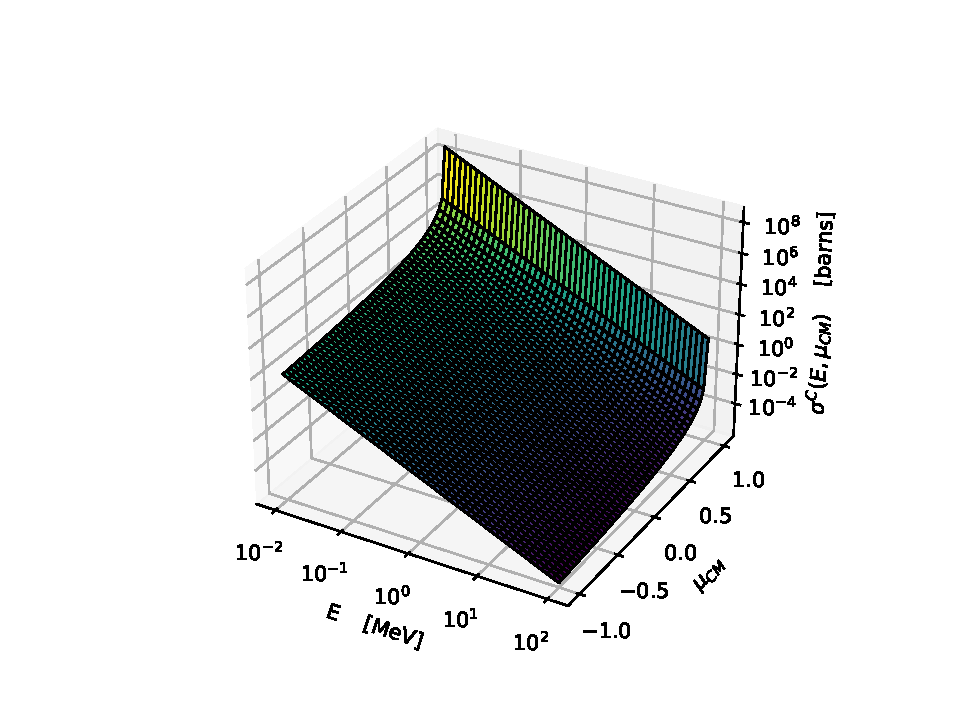
\includegraphics[scale=1.00]{../figures/chapter-4/sigma-C.pdf}
    \caption{Distinguishable Coulomb differential cross section for energetic deuterons colliding with background tritons cutoff at $\mucm = 0.99$}
    \label{fig:sigma_c}
\end{figure}

The total scattering cross section associated with Eq. \eqref{eqn:coulomb-dcs} is found by integrating over $\mucm$ from $-1$ to some cutoff angle, $\mu_{cut}$ resulting in the following total scattering cross section
\begin{equation} \label{eqn:unscreened-total-xs}
    \sigma^C_d(E) = \left(\dfrac{Z_1^2 \, Z_2^2 \, \left(\alpha \, \hbar c\right)^2}{ 4 \, E^2 \, \left(\frac{A}{1 + A} \right)^2}\right) \dfrac{\mu_{cut}}{1-\mu_{cut}}, \quad \text{where} \,\, -1 < \mu_{cut} < 1.
\end{equation}
Figure \ref{fig:sigma_c_total} shows Eq. \eqref{eqn:unscreened-total-xs} for several different collisions and with a cutoff cosine of $\mu_{cut} = 0.999$. From Figure \ref{fig:sigma_c_total} as the energy of the incident particle increases the magnitude of the total cross section decreases, this can also be seen in Figure \ref{fig:sigma_c}. Additionally, as the mass of the incident particle increases so does the magnitude of the total cross section. Conversely, as the mass of the target particle increases, the magnitude of the of the total cross section decreases. Lastly, for nominal ICF energies, $<10$ MeV, the magnitude of Eq. \eqref{eqn:unscreened-total-xs} is large meaning that for typical ICF densities the mean free path is very small and highly peaked about zero angular deflection.
\begin{figure}[!htb]
    \centering
    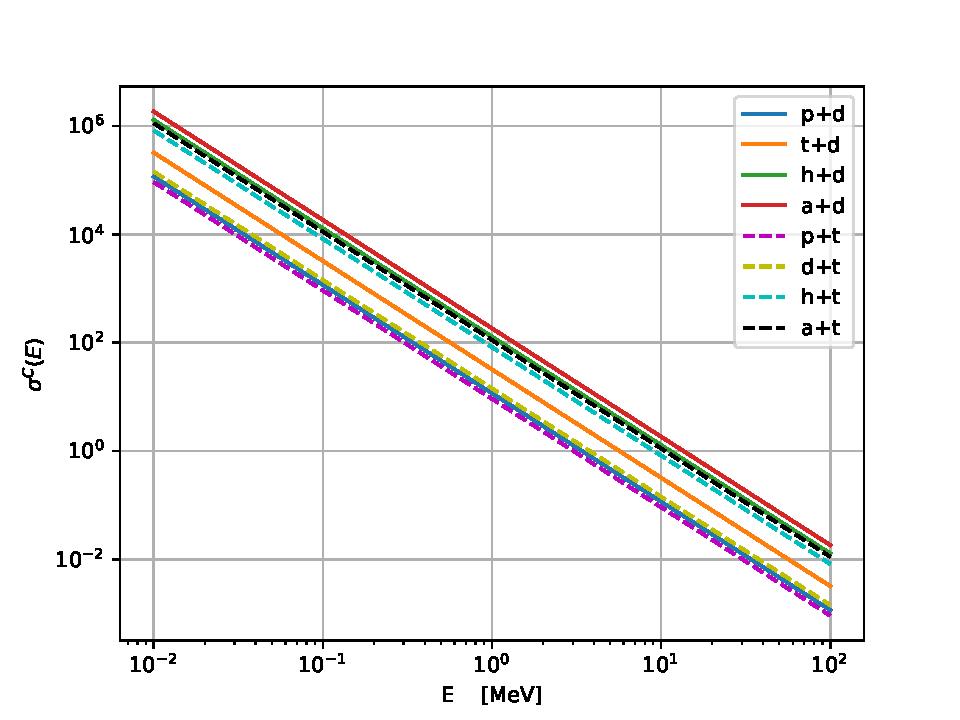
\includegraphics[scale=0.75]{../figures/chapter-4/total-sigma-C.pdf}
    \caption{Total distinguishable Coulomb differential cross section for several collisions cutoff at $\mucm = 0.999$}
    \label{fig:sigma_c_total}
\end{figure}

\subsubsection{Identical particles}
The identical particle unscreened Coulomb differential cross section is found by substituting Eq. \eqref{eqn:coulomb-scattering-amplitude} into Eq. \eqref{eqn:formula-identical-particles} giving,
\begin{multline} \label{eqn:coulomb-unscreened-identical}
   \sigma_{i}^{C} = \dfrac{\gamma^2}{k^2} \left[ \dfrac{1}{(1 - \mucm)^2} + \dfrac{1}{(1 + \mucm)^2} \right. \\ \left. + \dfrac{(-1)^{2s}}{2s+1} \dfrac{2}{(1 - \mucm)(1 + \mucm)} \cos \left( \gamma \, \log \, \dfrac{1 - \mucm}{1 + \mucm} \right) \right].
\end{multline}
Figure \ref{fig:coulomb-identical} shows $\sigma_{C,i}$ for a variety of incident particle energies and cosine of CM scattering angles. In Figure \ref{fig:coulomb-identical} it is clear that the identical particle Coulomb differential cross section is highly peaked about $\mucm = -1, 1$. When comparing the distinguishable and identical differential cross sections we see that both differential cross section are highly peaked about $\mucm = 1$ meaning that it is highly likely that the initial particle will scatter in the forward direction in both identical and distinguishable collisions; however, the identical particle differential cross section is highly peaked about $\mucm = -1$ meaning that it is very likely that the incident particle will transfer all of it's energy to the target particle. This means that the recoil now looks exactly like the incident particle underwent a small angle deflection collision.
\begin{figure}[!htb]
    \centering
    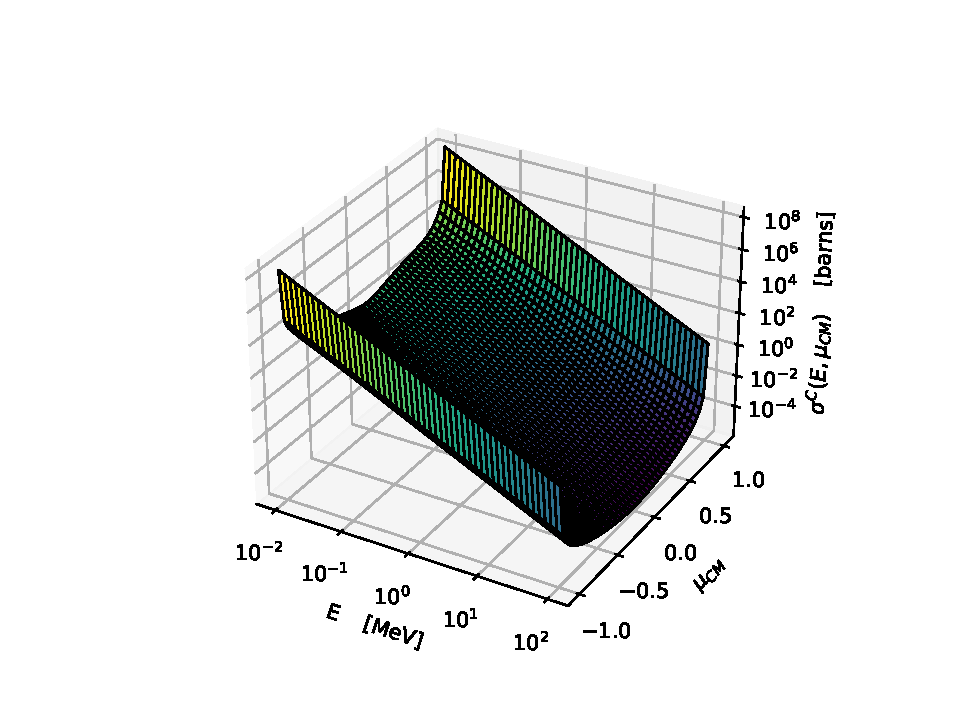
\includegraphics[scale=1.00]{../figures/chapter-4/sigma-Ci.pdf}
    \caption{The identical particle Coulomb differential cross section for deuterons colliding with background deuterons for $\mucm = [-0.99,0.99]$}
    \label{fig:coulomb-identical}
\end{figure}

Eq. \eqref{eqn:coulomb-unscreened-identical} can be greatly simplified when $\gamma \ll 1$ meaning that the velocity of the incident particle is so large that $\hbar v \gg Z_1 Z_2 e^2$. In this case the cosine in the third term can be replaced by unity and Eq. \eqref{eqn:coulomb-unscreened-identical} becomes
\begin{equation} \label{eqn:coulomb-unscreened-identical-simplified}
   \sigma_{i}^{C} \approx \dfrac{2 \, \gamma^2}{k^2 (1 - \mucm^2)} \left[\dfrac{1+ \mucm^2}{1-\mucm^2} + \dfrac{(-1)^{2s}}{2s+1}\right], \quad \text{when} \,\, \gamma \ll 1.
\end{equation}
For the opposite case, $\hbar v \ll Z_1 Z_2 e^2$, the cosine term in Eq. \eqref{eqn:coulomb-unscreened-identical} is a rapidly oscillating function, and the resulting cross section differs significantly from the Rutherford value given by Eq. \eqref{eqn:coulomb-unscreened-identical-simplified}. Figure \ref{fig:coulomb-identical-2d} shows the oscillations in the differential cross section due to the cosine term at various incident particle energies. In Figure \ref{fig:coulomb-identical-2d} it is clear that at low energies ($E < 10$ keV) these oscillations are significant; however, at higher energies these oscillations atr not significant and the Eq. \eqref{eqn:coulomb-unscreened-identical} rapidly approaches Eq. \eqref{eqn:coulomb-unscreened-identical-simplified}.

\begin{figure}[!htb]
    \centering
    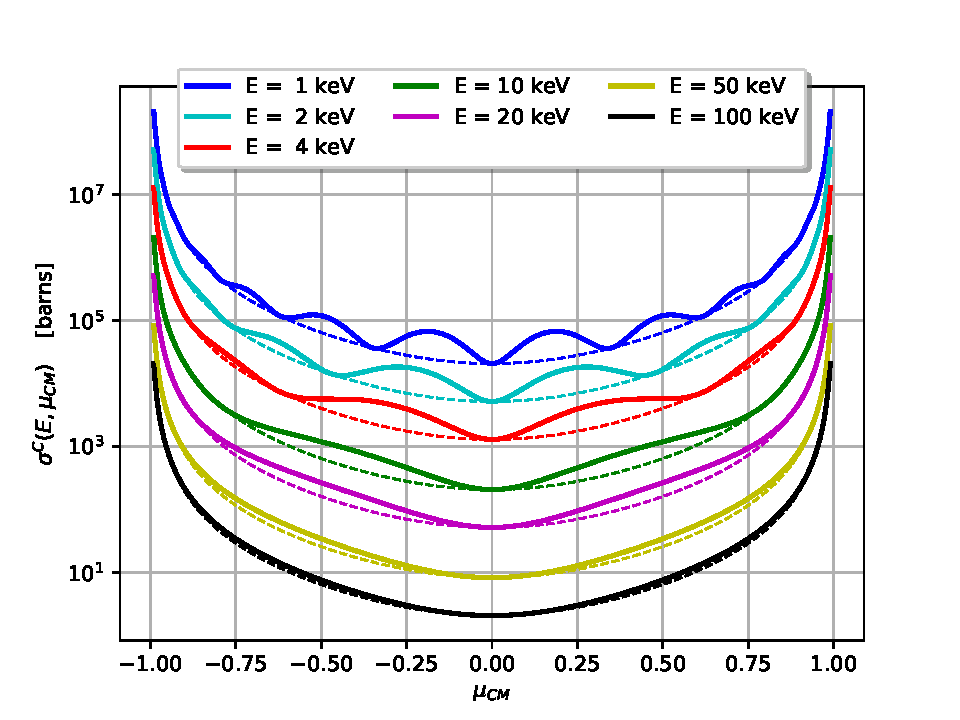
\includegraphics[scale=0.75]{../figures/chapter-4/sigma-Ci-2d.pdf}
    \caption{Comparison between the full (solid lines) and approximate (dashed lines) identical particle Coulomb differential cross sections at various energies for tritons colliding with background tritons for $\mucm = [-0.99,0.99]$.}
    \label{fig:coulomb-identical-2d}
\end{figure}

% ------------------------------------------------
% SCREENING FUNCTIONS 
% ------------------------------------------------
\subsubsection{The Yukawa Potential}
Here the Yukawa potential is introduced as a reasonable form of screening in plasmas. To introduce the concept of Debye shielding consider a finite temperature plasma consisting of a statistically large number of electrons and ions and by assuming that the ion and electron densities are initially equal and spatially uniform. The ions and electrons in the background plasma have random thermal motion, thermally induced pertubations about the equilibrium will cause small, transient spatial variations of the electrostatic potential $\phi$. Next, the following assumptions are made:
\begin{enumerate}
    \item The background plasma is assumed to be nearly collisionless so that collisions between particles may be neglected
    \item Each species, denoted as $i$, may be considered as a ``fluid'' having a density $n_i$, and a temperature $T_i$, a pressure $P_i = n_i \kappa T_i$, and a mean a velocity $\boldsymbol{u}_i$ so that the collisionless equation of motion for each fluid is
    \begin{equation} \label{eqn:collisionless-motion}
        m_i \dfrac{d \boldsymbol{u}_i}{dt} = q_i \boldsymbol{E} - \dfrac{1}{n_i} \nabla P_i
    \end{equation}
    where $m_i$ is the particle mass, $q_i$ is the charge of a particle, and $\boldsymbol{E}$ is the electric field.
\end{enumerate}

Now consider a perturbation with a sufficiently \textit{slow} time dependence to allow the following assumptions:
\begin{enumerate}
    \item The inertial term $\approx d/dt$ on the left-hand side Eq. \eqref{eqn:collisionless-motion} is negligible and may be dropped.
    \item Inductive electric fields are negligible so the electric field is almost entirely electrostatic, i.e., $\boldsymbol{E} \approx - \nabla \phi$.
    \item All temperature gradients are smeared out by thermal particle motion so that the temperature of each species is spatially uniform
    \item The plasma remains in thermal equilibrium throughout the perturbation
\end{enumerate}
Invoking these approximations, Eq. \eqref{eqn:collisionless-motion} reduces to
\begin{equation} \label{eqn:pressure-balance}
    0 \approx -n_i q_i \nabla \phi - \kappa T_i \nabla n_i,
\end{equation}
which is a simple balance equation between the force due to the electrostatic electric field and the force due to the isothermal pressure gradient. Eq. \eqref{eqn:pressure-balance} is readily solved to give the Boltzmann relation
\begin{equation} \label{eqn:boltzmann-relation}
    n_i = n_{i,0} \exp\left(-q_i \phi / \kappa T_i\right),
\end{equation}
where $n_{i,0}$ is a constant. It is important to note that Eq. \eqref{eqn:boltzmann-relation} results from the assumption that the perturbation is \textit{very slow}; if this is not the case, then inertial effects, inductive electric fields, or temperature gradient effects will cause the plasma to have completely different behavior than the Boltzmann relation.

Next, imagine \textit{slowly} inserting a single additional particle with charge $q_T$ into an initially unperturbed, spatially uniform, neutral plasma. To keep the algebra simple, the origin of the coordinate system is defined to be at the location of the test particle. Before insertion of the test particle, the plasma potential was $\phi = 0$ everywhere because the ion and electron densities were spatially uniform and equal, but now the ions and electrons will be perturbed because of their interaction with the test particle. Particles having the same polarity as $q_T$ will be slightly repelled whereas particles of opposite polarity will be slightly attracted. This slight displacement resulting from these repulsions and attractions will result in a small, but finite, potential in the plasma.

This slight displacement of plasma particles is called \textit{shielding} or \textit{screening} of the test particle because the displacement tends to reduce the effectiveness of the test particle field. As an example, suppose the test particle is a positively charged ion which when inserted into the plasma attracts the nearby electrons and repels the ions. The net result is a negative charge cloud surrounding the test particle which effectively shields the test particles potential from the rest of the plasma.

The screening effect is calculated using Poisson's equation with the source terms being the test particle and its associated cloud. The cloud contribution is determined using the Boltzmann relation for the particles that participate in the screening. This is a ``self-consistent'' calculation for the potential because the shielding cloud is affected by its self-potential.

Thus, Poisson's equation becomes
\begin{equation} \label{eqn:poisson-relation}
    \nabla^2 \phi = - \dfrac{1}{\epsilon_0} \left[q_T \delta(\boldsymbol{r}) + \sum\limits_{i} n_i(\boldsymbol{r}) q_i\right],
\end{equation}
where the term $q_T \delta(\boldsymbol{r})$ on the right-hand side represents the charge density due to the test particle and the term $\sum\limits_{i} n_i(\boldsymbol{r}) q_i$ represents the charge density of all plasma particles that participate in the screening. Because the test particle was inserted slowly, the plasma response will be Boltzmann-like and we may substitute Eq. \eqref{eqn:boltzmann-relation} into Eq. \eqref{eqn:poisson-relation}. Additionally, because the perturbation due to a single test particle is infinitesimal, it can be assumed that $|q_i \phi| \ll \kappa T_i$, reducing Eq. \eqref{eqn:poisson-relation} to 
\begin{equation} \label{eqn:poisson-relation-2}
    \nabla^2 \phi = - \dfrac{1}{\epsilon_0} \left[q_T \delta(\boldsymbol{r}) + \sum\limits_{i} n_{i,0} q_i \left(1 - \dfrac{q_i \phi}{\kappa T_i}\right) \right]
\end{equation}
The assumption of initial neutrality means that $n_{e0}q_e + \sum\limits_{i} n_{i,0} q_i = 0$, in which case Eq. \eqref{eqn:poisson-relation-2} reduces to
\begin{equation} \label{eqn:poisson-relation-3}
    \nabla^2 \phi - \dfrac{1}{\lambda_D^2} \phi = - \dfrac{q_T}{\epsilon_0} \delta(\boldsymbol{r})
\end{equation}
where the effective Debye length is defined by
\begin{equation}
    \dfrac{1}{\lambda_D^2} = \sum\limits_i \dfrac{1}{\lambda_i^2}
\end{equation}
and the species Debye length $\lambda_i$ is
\begin{equation}
    \lambda_i^2 = \dfrac{\epsilon_0 \kappa T_i}{n_{i0}q_i^2}.
\end{equation}
Finally Eq. \eqref{eqn:poisson-relation-3} can be solved to give
\begin{equation} \label{eqn:yukawa-potential}
    \phi(\boldsymbol{r}) = \dfrac{q_T}{4 \pi \epsilon_0 r} \text{e}^{-r/\lambda_D};
\end{equation}
this is sometimes called the Yukawa potential. In Eq. \eqref{eqn:yukawa-potential} the exponential term decreases more rapidly than the $1/r$ term thereby making the probability that particles will experience interactions at distances much greater than $R$ impossible. This leads to an interaction potential that is finite as $r \rightarrow \infty$ while still possessing the same general behavior as the original Coulomb interaction potential.

% ------------------------------------------------
% SCREENED COULOMB DIFFERENTIAL CROSS SECTIONS 
% ------------------------------------------------
\subsubsection{Screened coulomb differential cross sections}
Using the Yukawa potential derived in the previous section, the screened Coulomb differential cross section can be derived. The Schr\"{o}dinger equation with the Yukawa potential cannot be solved exactly and therefore its solution is approximated with the Born approximation. The Born approximation consists of approximating the the scattered wave function by a plane wave, and gives the following formula for the scattering amplitude
\begin{equation} \label{eqn:first-born-approximation}
    f(\theta) \approx - \dfrac{2 \, m}{\hbar^2} \int\limits_0^{\infty} U(r) \, \dfrac{\sin qr}{q} \, r \, dr
\end{equation}
where $q = 2 \, k \, \sin \theta / 2$. Substituting the screened interaction potential into Eq. \eqref{eqn:first-born-approximation} and yields
\begin{equation} \label{eqn:wentzel-scattering-amplitude}
    f_s(\theta) = \dfrac{Z_1 \, Z_2 \, e^2 \, m}{2 \, k^2 \, \hbar^2} \dfrac{1}{(2kR)^{-2} + \sin^2 \theta/2} = \dfrac{\gamma}{2 \, k} \left[\dfrac{1}{(2kR)^{-2} + \sin^2 \theta/2}\right].
\end{equation}
In Eq. \eqref{eqn:wentzel-scattering-amplitude} the term $(2kR)^{-2}$ is often referred to as the screening parameter and is denoted by $A_s$. Note that as $A_s \rightarrow 0$ Eq. \eqref{eqn:wentzel-scattering-amplitude} approaches the unscreened Coulomb potential scattering amplitude, Eq. \eqref{eqn:Coulomb_potential}, without the exponential and gamma function terms. In fact it has been shown that the Born approximation is not a valid approximation of the scattering amplitude when a screened interaction potential is used for nucleon-nucleon interactions unless the incident particles energy is at relativistic speeds. Nonetheless, the differential cross sections for distinguishable and identical particles are derived using Eq. \eqref{eqn:wentzel-scattering-amplitude} as they result in differential cross sections that are at least finite at $\mucm = 1$ and resemble the Coulomb differential cross sections previously derived.

Using Eqs. \eqref{eqn:formula-distinguishable-particles} and \eqref{eqn:formula-identical-particles} the screened Coulomb differential cross section for distinguishable and identical particles are
\begin{equation} \label{eqn:screened-coulomb-d}
    \sigma_{d}(E,\mucm) = \dfrac{\gamma^2}{k^2} \dfrac{1}{\left[A_s + 1 - \mucm\right]^2},
\end{equation}
and
\begin{multline} \label{eqn:screened-coulomb-i}
    \sigma_{i}(E,\mucm) = \dfrac{\gamma^2}{k^2} \left[ \dfrac{1}{\left(A_s + 1 - \mucm\right)^2} + \dfrac{1}{\left(A_s + 1 + \mucm\right)^2} \right. \\ \left. + \dfrac{(-1)^{2s}}{2s+1} \dfrac{2}{\left(A_s + 1 - \mucm\right)\left(A_s + 1 + \mucm\right) }\right].
\end{multline}
In Eq. \eqref{eqn:screened-coulomb-d} as $A_s \rightarrow 0$ it becomes the unscreened Coulomb differential cross sections (Eq. \eqref{eqn:coulomb-dcs}). However, in the identical particle case as $A_s \rightarrow 0$ instead of approaching the unscreened identical particle differential cross Eq. \eqref{eqn:screened-coulomb-i} becomes the approximate unscreened identical particle differential cross section (Eq. \eqref{eqn:coulomb-unscreened-identical-simplified}). This discrepancy is due to the validity of the Born approximation, which is only valid if the incident particle has high energy. However, Eqs. \eqref{eqn:screened-coulomb-d} and \eqref{eqn:screened-coulomb-i} are considered ``good enough'' approximations to the true differential cross section and are used throughout the remainder of this dissertation. 



% ------------------------------------------------
% NES DIFFERENTIAL CROSS SECTIONS 
% ------------------------------------------------
\subsection{Nuclear Elastic Scattering}
Nuclear elastic scattering collisions are short-range collisions that can result in large angular deflections. The NES differential cross sections are expressed in terms of Legendre moments,
\begin{equation} \label{eqn:nes_differential cross section}
    \sigma_{x,t \rightarrow x}^N(E^{\prime} \rightarrow E; \mucm) = \sum_{l=0}^L \dfrac{2l+1}{2} b_l(E^{\prime}) P_l(\mucm),
\end{equation}
where $P_l(\mucm)$ are the Legendre polynomials of order $l$, and $b_l(E)$ are the tabulated Legendre expansion coefficients \cite{Brown-2018}.

Figure \ref{fig:nesTotal} shows the total NES cross sections for DD, DT, DH, and DA collisions. In Figure \ref{fig:nesTotal}, as the energy of the incident particle increases so does the total NES cross sections. These NES cross sections are much smaller in magnitude than the corresponding Coulomb cross sections at low incident energies, $\sim 10^4$ barns at $0.1 \mev$. However, at high energies, $(> 1 \mev)$, the NES and Coulomb cross sections become comparable in magnitude with the Coulomb cross section varying between $10^2$ and $10^0$ barns between incident particle energies of $1 \mev$ and $10 \mev$. In general then, the slowing down of low energy particles $(< 1 \mev)$ is dominated by Coulomb collisions whereas the slowing down of energetic particles $(> 1 \mev)$ is caused by a combination of both Coulomb and NES collisions.

\begin{figure}[!htb]
    \centering
    \includegraphics[scale=0.75]{../figures/chapter-4/sigmaNES_total.pdf}
    \caption{Total nuclear elastic scattering cross sections}
    \label{fig:nesTotal}
\end{figure}

In Figure \ref{fig:nesDCS} the NES differential cross section for the DT collision is shown at various incident particle energies. From Figure \ref{fig:nesDCS}, at low incident particle energies the scattering is approximately isotropic; however, at high energies there is a significant probably of scattering in backward directions. Scattering in backward directions causes the particles to lose a significant amounts of energy in single collisions. Therefore at high energies there is a significant probability that a particle will lose a considerable amount of energy causing it to slow down quicker than if only Coulomb collisions are taken into account. Nakao et al. \cite{Nakao-1990} examined the effects of NES on the slowing down of energetic light ions in ICF plasmas and found that they contributed significantly for high energy, $(> 10 \mev)$, protons slowing down in a DT plasma.

\begin{figure}[!htb]
    \centering
    \includegraphics[scale=0.75]{../figures/chapter-4/sigmaNES_dcs.pdf}
    \caption{Nuclear elastic scattering differential cross section for DT}
    \label{fig:nesDCS}
\end{figure}

% ------------------------------------------------
% INTERFERENCE DIFFERENTIAL CROSS SECTIONS 
% ------------------------------------------------
\subsection{Interference differential cross sections}
The interference differential cross section describes the quantum mechanical interference between the long range Coulomb collisions and the short range NES collisions \cite{Hale-1983}. R-matrix theory is used to describe these interference cross sections as it allows for a parametric treatment of the short ranged (NES) effects, while accounting exactly for the long-ranged (Coulomb) effects. Therefore an accurate total elastic scattering differential is developed that is constrained by a theory that embodies the fundamental properties of nuclear interactions and ensures the correct limiting behavior at small angles and low energies, where the long-ranged effects dominate.

Screened interference differential cross sections for distinguishable particles are given by,
\begin{equation} \label{eqn:interfenceDistinguishable}
    \sigma_d^I(E,\mucm) = \dfrac{-2 \, \eta}{1 - \mucm + A_s} \Re \left\lbrace \exp \left[ i \eta(E) \ln \left( \dfrac{1 - \mucm + A_s}{2} \right) \right]\sum\limits_{\ell = 0}^L \dfrac{2\ell + 1}{2} a_{\ell}(E) P_{\ell}(\mucm) \right\rbrace
\end{equation}
where $a_{\ell}(E)$ are the complex coefficients for expanding the trace of the nuclear scattering amplitude matrix \cite{Brown-2018}. Similarly the screened interference differential cross section for identical particles is,
\begin{multline} \label{eqn:interfenceIdentical}
    \sigma_i^I(E,\mucm) = \dfrac{-2 \, \eta}{\left(1 - \mucm + A_s\right)\left(1 + \mucm + A_s\right)} \\
    \times \Re \left\lbrace \sum\limits_{\ell = 0}^L \dfrac{2 \ell + 1}{2} a_{\ell}(E) P_{\ell}(\mucm) \left[ \left(1 + \mucm + A_s \right) \exp\left(i \eta \ln \dfrac{1 - \mucm + A_s}{2}\right) \right.\right. \\ \left.\left. + (-1)^{\ell} \left(1 - \mucm + A_s \right) \exp\left(i \eta \ln \dfrac{1 + \mucm + A_s}{2}\right) \right]\right\rbrace.
\end{multline}
Eqs. \eqref{eqn:interfenceDistinguishable} and \eqref{eqn:interfenceIdentical} result in differential cross sections that oscillate between positive and negative values. Negative cross sections do not make physical sense, and therefore interference cross sections only make sense in combination with the Coulomb and NES cross sections such that the total cross section remains positive.

Figure \ref{fig:interferenceTotal} shows total interference differential cross sections for deuteron-deuteron, deuteron-triton, deuteron-helion, and deuteron-$\alpha$ particle collisions. In Figure \ref{fig:interferenceDCS} the cross sections vary in amplitude between positive and negative values across the entire range of energies. Additionally, at high energies the magnitude of the cross section becomes comparable to the magnitudes of the Coulomb and NES cross sections suggesting that the interference cross section plays a significant role in slowing down of high energy ions.
\begin{figure}[!htb]
    \centering
    \includegraphics[scale=0.65]{../figures/chapter-4/sigmaI_total.pdf}
    \caption{Total interference elastic scattering cross sections}
    \label{fig:interferenceTotal}
\end{figure}

In Figure \ref{fig:interferenceDCS}, the deuteron-triton differential cross section is plotted versus the cosine of the CM scattering angle for several incident ion energies. For all energies as $\mucm \rightarrow 1$ the differential cross section is seen to oscillate rapidly between increasing large positive and negative values. This oscillation is due to the exponential and logarithmic terms in Eqs. \eqref{eqn:interfenceDistinguishable} and \eqref{eqn:interfenceIdentical} which are oscillating with increasing frequency between positive and negative values.
\begin{figure}[!htb]
    \centering
    \includegraphics[scale=0.5]{../figures/chapter-4/sigmaI_dcs.pdf}
    \caption{Differential interference elastic scattering cross sections}
    \label{fig:interferenceDCS}
\end{figure}

% ------------------------------------------------
% FOKKER-PLANCK MOMENTS
% ------------------------------------------------
\subsection{Fokker-Planck Moments}

\subsubsection{Stopping powers}

\subsubsection{Angular moments}

\subsubsection{Energy moments}

% ------------------------------------------------
% NUCLEAR REACTION DIFFERENTIAL CROSS SECTIONS 
% ------------------------------------------------
\section{Thermonuclear Reactions}
Thermonuclear (TN) reactions are collisions that cause the identities of the emitted particles to differ from the incident and target particles. There are 4 main nuclear reactions of interest in ICF applications which are typically reffered to as the big 4, they are:
\begin{multicols}{2}
\begin{itemize}
    \item $\ce{^{2}_{1}H} \, (t, \, n)\, \ce{^{4}_{2}He}$  $(Q = 10.0 \mev)$
    \item $\ce{^{3}_{2}He}\, (d, \, p)\, \ce{^{4}_{2}He}$  $(Q = 10.0 \mev)$
    \item $\ce{^{2}_{1}H} \, (d, \, n)\, \ce{^{3}_{2}He}$  $(Q = 10.0 \mev)$
    \item $\ce{^{2}_{1}H} \, (d, \, p)\, \ce{^{3}_{1}H}$   $(Q = 10.0 \mev)$
\end{itemize}
\end{multicols}
where $Q$ is the Q-value of the reaction. The three reacting isotopes, (d,t,h), produce seven charged particle products plus two neutron products. TN reactions cause the energy spectrum of charged particles and neutrons to vary from thermal background temperatures all the way up to $\sim 30 \mev$. TN reactions are typically divided into primary reactions, and secondary reactions (fusion of a primary product). In addition, tertiary interactions utilizing both processes in sequence can produce particles with the highest energy.  

Figure \ref{fig:tnTotal} shows the total TN reaction cross sections for the major four reactions. In Figure \ref{fig:tnTotal} we see that the TN reaction with the highest probability is the deuterium-tritium reaction with a peak at $0.1 \mev$ of $\sim 4 \barns$. The next largest TN reaction is the deuterium-helion reaction with a peak at $0.4 \mev$ of $\sim 1 \barns$; however, most ICF background plasmas do not contain appreciable amounts of $\ce{^{3}_{2}He}$ and therefore this reaction is considered a secondary reaction because only helions produce from deuterium-deuterium reactions can produce the necessary helions. The two deuterium-deuterium reactions occur with roughly equal probability. It is also worth noting that at high energies ($> 2 \mev$) all the TN reactions occur with equal probability.

\begin{figure}[!htb]
    \centering
    \includegraphics[scale=0.75]{../figures/chapter-4/tnTotal.pdf}
    \caption{Total thermonuclear reaction cross sections}
    \label{fig:tnTotal}
\end{figure}

Figure \ref{fig:tnDiffernetialCrossSections} shows the angular dependence of the TN differential cross sections at various energies for the DD and DT reactions. From Figure \ref{fig:tnDiffernetialCrossSections}, the neutron emitted in the DT reaction is emitted fairly isotopically at low energies. However, as the energy of the incident deuteron increases, the outgoing neutron is increasingly more likely to emitted in forward directions. Similarly, in the DD reaction there is slight bias in the forward direction at low incident particle energies and increases with increasing incident particle energy. In general, it can be concluded in TN reactions that the light particle tends to scatter in forward directions while the heavy particle will scatter in backward directions.

\begin{figure}[!htb]
  \centering
  \begin{subfigure}{.45\textwidth}
    \centering
    \includegraphics[scale=0.45]{../figures/chapter-4/ddDCS.pdf}
    \caption{$d + d \rightarrow p + h$}
    \label{fig:ddDCS}
  \end{subfigure}%
  \begin{subfigure}{.45\textwidth}
    \centering
    \includegraphics[scale=0.45]{../figures/chapter-4/dtDCS.pdf}
    \caption{$d + t \rightarrow n + a$}
    \label{fig:dtDCS}
  \end{subfigure}
  \caption{Thermonuclear reaction differential cross sections}
  \label{fig:tnDiffernetialCrossSections}
\end{figure}

% ------------------------------------------------
% ELECTRONIC ELASTIC SCATTERING
% ------------------------------------------------
\section{Electronic stopping powers}

\end{document}
